\documentclass[11pt, oneside]{article}   	% use "amsart" instead of "article" for AMSLaTeX format
\usepackage{geometry}                		% See geometry.pdf to learn the layout options. There are lots.
\geometry{letterpaper}                   		% ... or a4paper or a5paper or ... 
%\geometry{landscape}                		% Activate for for rotated page geometry
%\usepackage[parfill]{parskip}    		% Activate to begin paragraphs with an empty line rather than an indent
\usepackage{graphicx}				% Use pdf, png, jpg, or eps� with pdflatex; use eps in DVI mode
								% TeX will automatically convert eps --> pdf in pdflatex		
\usepackage{amssymb}
\usepackage{amsmath}
\usepackage{parskip}
\usepackage{color}
\usepackage{hyperref}

\title{Problem}
%\author{The Author}
%\section{}
%\subsection*{}
\usepackage{listings}

\date{}							% Activate to display a given date or no date

\graphicspath{{/Users/telliott_admin/Dropbox/Tex/png/}}
% \begin{center} 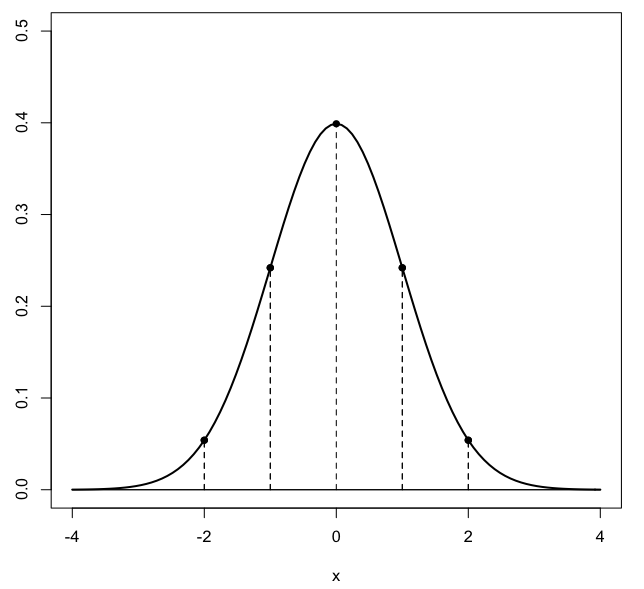
\includegraphics [scale=0.4] {gauss3.png} \end{center}
\begin{document}
\maketitle
\Large
I came across the following problem (edited slightly):

A deck of n different cards is shuffled and laid on the table next to your left hand, face down. An identical deck of cards, independently shuffled, is laid at your right hand, also face down. You start turning up cards at the same rate with both hands, first the top card from both decks, then the next-to-top cards from both decks, and so on. What is the probability that you will simultaneously turn up identical cards from the two decks? 

Suppose we start with the $13$ spades, or with the $26$ red cards (hearts plus diamonds).  A standard deck has $52$ cards.  Suppose we mark the two decks somehow to allow $n = 52 \times k$. The answer to the question about probability should depend on n. As n gets very large what happens to this probability? Does it converge to 0? Or to 1?

\subsection*{solution}
Suppose we run through the whole deck and don't get a match.  That is certainly possible---to see this, just order the spades in reversed order.

\texttt{AKQJT98765432}

\texttt{23456789TJQKA}

and then, since $n$ is odd, swap the $8$ from one deck with \emph{any other card} in the same deck.  If the number of cards $n$ had been even, no swap would be needed.  

To construct a "no-match" situation using two randomly shuffled decks, proceed as follows.  Find all the positions where the two decks do match, and for each pair of matching positions, exchange the relevant cards in one of the decks.  If the number of matches was odd, at the end, take the last match and do an exchange with \emph{any other card} in the same deck. 

For any single comparison with a randomly shuffled standard deck, the probability of not matching is $51/52$ and the probability of not matching on all 52 comparisons is
\[ \frac{51}{52} \times \frac{51}{52} \times \frac{51}{52} \dots \times \frac{51}{52} \ \ \ \ \ \ \text{(52 terms)} \]
\[ = \frac{51}{52}^{52} \approx 0.36 \]
The probability of matching for at least one comparison is $1$ minus that, which is certainly not $1$.

Now, I notice two things.  First, I computed
\[ \ [ \ \frac{(n-1)}{n} \ ] ^n \]
for various values of $n$, and found that the result changes only a little as $n$ gets larger.  Using Python:
\begin{lstlisting}[language=Python]
>>> def f(n):
...     return ((n-1)*1.0/n)**n
... 
>>> f(20)
0.358485922409
>>> f(52)
0.36431351956896996
>>> f(1000000)
0.36787925722106646
\end{lstlisting}
The second thing is that this value $0.36 \dots$ looks suspiciously familiar.  A little investigation reveals that it is equal to $1/e$.

\begin{lstlisting}[language=Python]
>>> from math import e
>>> e
2.718281828459045
>>> 1/e
0.36787944117144233
>>>
\end{lstlisting}

The reason turns out to be pretty simple.  Our formula was 
\[ (\frac{n-1}{n})^n \]
and this can be rearranged to: 
\[ (1 - \frac{1}{n})^n \]
Recall the Maclaurin series for $e^x$:
\[ e^x = 1 + x + \frac{x^2}{2!} + \dots \]
Thus, a good approximation is $e^x \approx 1 + x$ for small $x$.  So
\[ e^{-x} \approx 1 - x \]
\[ e^{-xp} \approx (1-x)^p \]
Hence
\[ (1 - \frac{1}{n})^n \approx e^{(-1/n)\ n } = e^{-1} \]
As $n$ gets large, $1/n$ gets smaller, and the approximation continues to improve.
\end{document} 